\chapter{Aplikasi Sensus Penduduk Menggunakan Trigger dan views}
\section{Resume Langkah-Langkah Proses Login Apex}
\par
\begin{enumerate}
    \item Pertama kunjungi Aplikasi APEX Online di \textit{https://apex.oracle.com/} 
    \begin{figure}[!htbp]
    \centering
    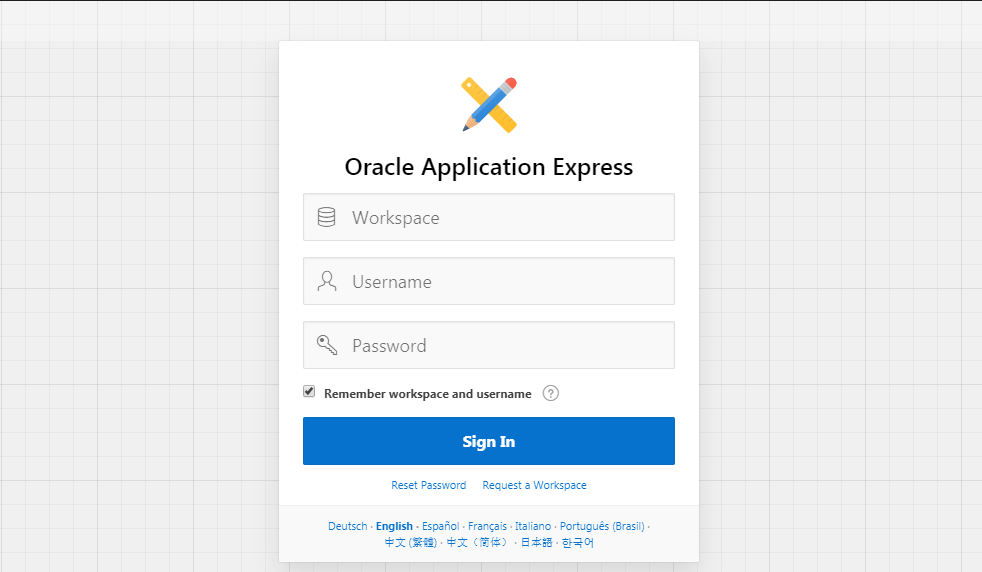
\includegraphics[width=13cm,height=8cm]{figures/awal.PNG}
    \caption{Tampilan Sign In}
    \label{penanda}
    \end{figure}
    \item Kemudian Masuk pada APEX nya dengan Melakukan \textit{SIGN IN} jika tidak memiliki akun maka lakukan \textit{SIGN UP}.
    \item Lalu jika sudah masuk Aplikasi APEX nya maka akan muncul seperti gambar dibawah.
\begin{figure}[!htbp]
\centering
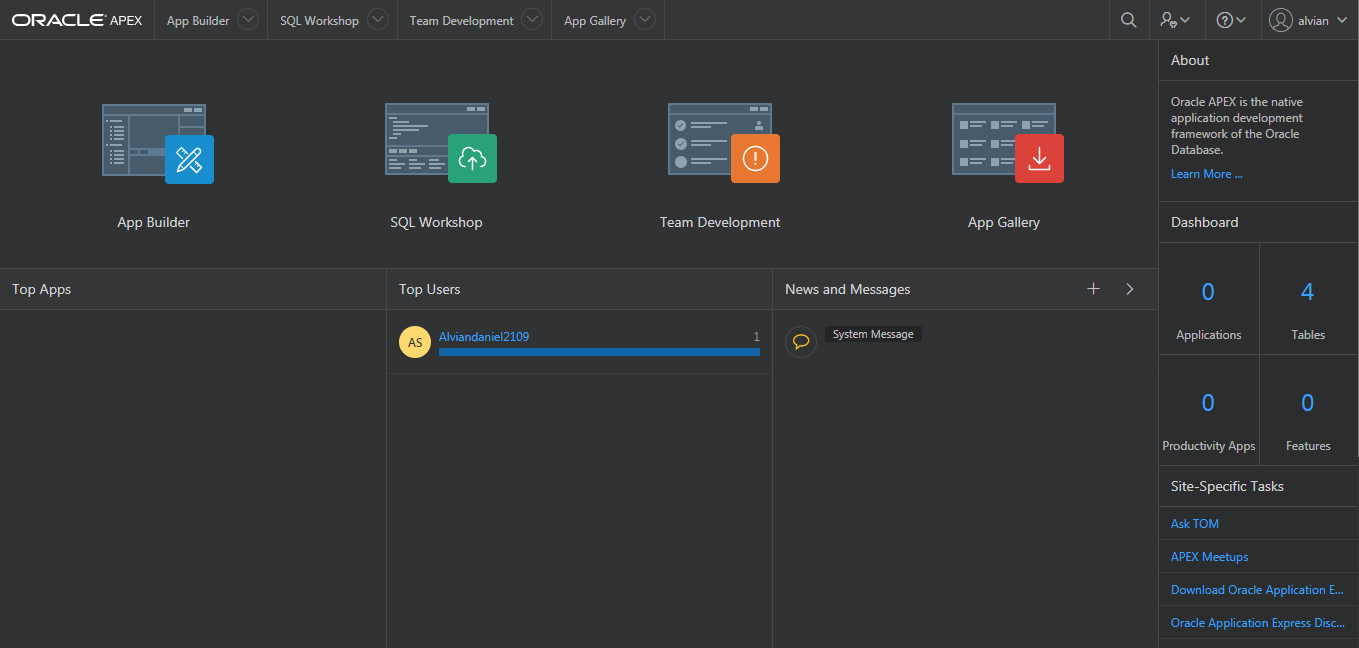
\includegraphics[width=13cm,height=9cm]{figures/awal1.PNG}
\caption{Menu Awal}
\label{penanda}
\end{figure}
    \item Kemudian Masuk Ke \textit{SQL WORKSHOP} lalu pilih \textit{SQL Commands}.
\begin{figure}[!htbp]
\centering
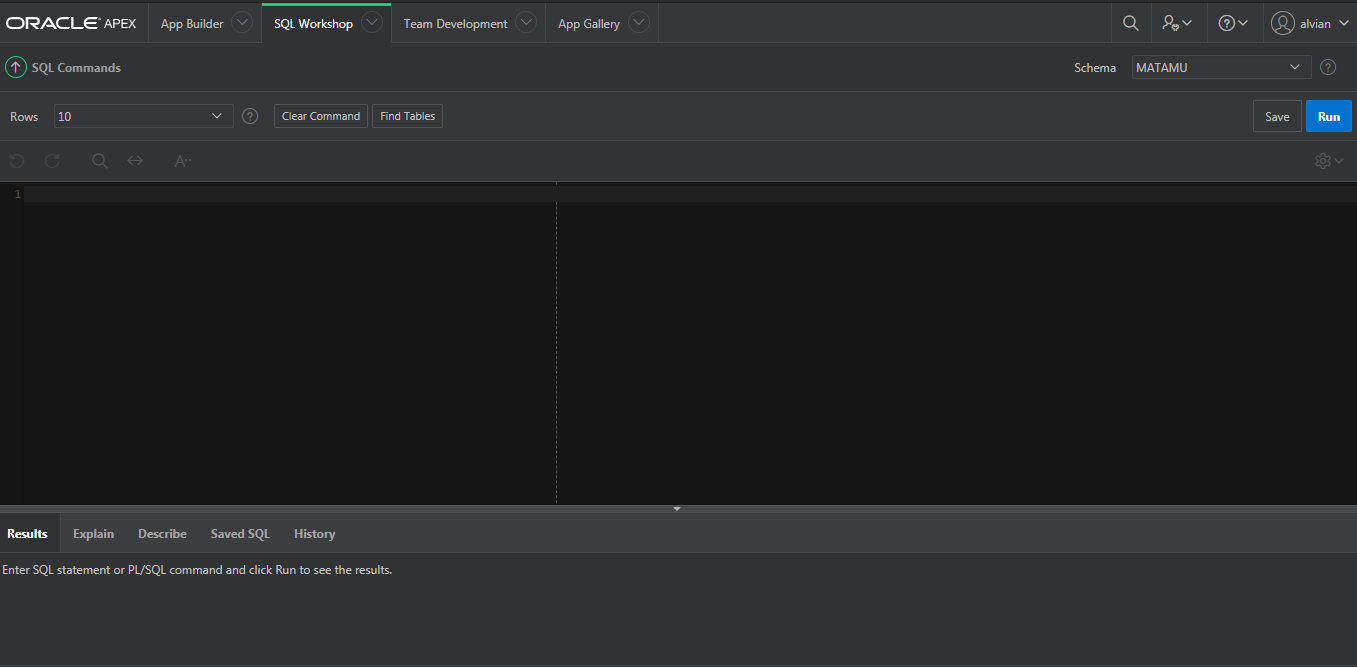
\includegraphics[width=13cm,height=9cm]{figures/B.PNG}
\caption{Halaman Commands}
\label{penanda}
\end{figure}

\section{Pembuatan Database Aplikasi.}
\item Pertama kita mulai dengan Membuat database baru, disini saya menggunakan 3 tabel (KK, STATUS, SENSUS JLH PENDUDUK)
\item Selanjutnya kita membuat tabel KK dan sudah ada Primary Key dalam tabel KK seperti gambar dibawah.
\begin{figure}[!htbp]
\centering
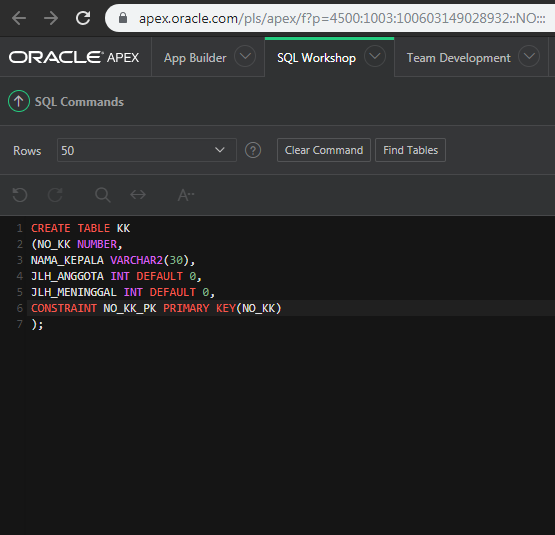
\includegraphics[width=13cm,height=7cm]{figures/C.PNG}
\caption{Tabel KK}
\label{penanda}
\end{figure}
\item Kemudian Kita membuat Tabel STATUS dan Primary Key seperti dibawah. 
\begin{figure}[!htbp]
\centering
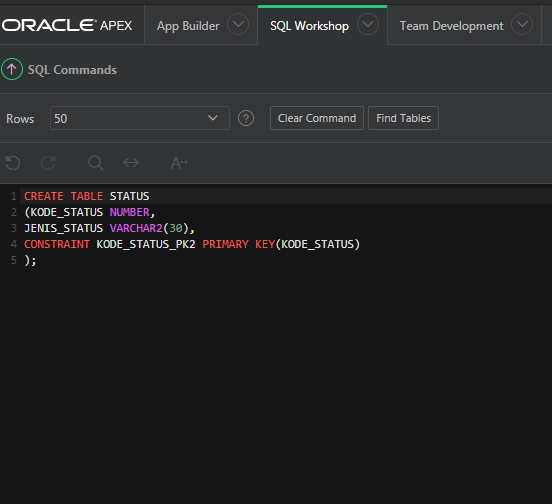
\includegraphics[width=13cm,height=7cm]{figures/D.PNG}
\caption{Tabel STATUS}
\label{penanda}
\end{figure}
\item Lalu, terakhir kita membuat tabel SENSUS JLH PENDUDUK beserta Primary key dan Foreign Key dari tabel KK dan STATUS.
\begin{figure}[!htbp]
\centering
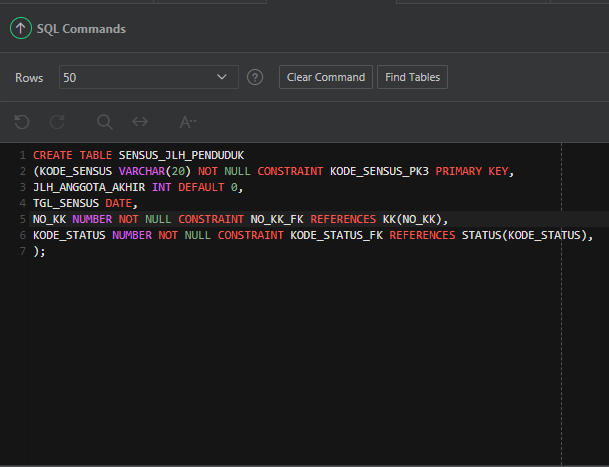
\includegraphics[width=13cm,height=7cm]{figures/E.PNG}
\caption{Tabel SENSUS}
\label{penanda}
\end{figure}
\item Setelah Kita membuat tabel Diatas lalu kita akan Melakukan Insert untuk memasukkan \textit{values} atau Record data.
\item Disini kita melakukan Insert pada tabel KK.
\begin{figure}[!htbp]
\centering
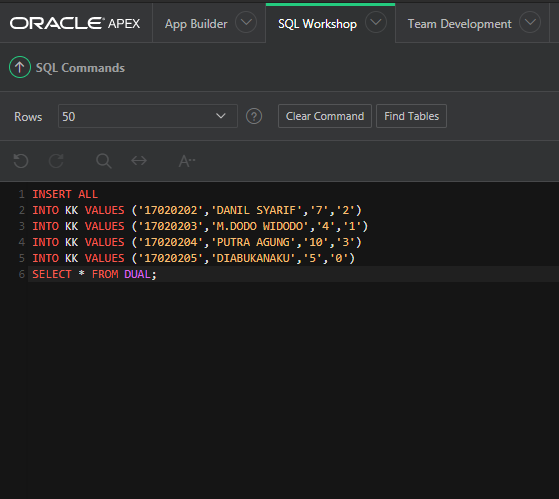
\includegraphics[width=13cm,height=7.5cm]{figures/F.PNG}
\caption{Insert Into tabel KK}
\label{penanda}
\end{figure}
\item Lalu, Kita melakukan Insert pada Tabel STATUS.
\begin{figure}[!htbp]
\centering
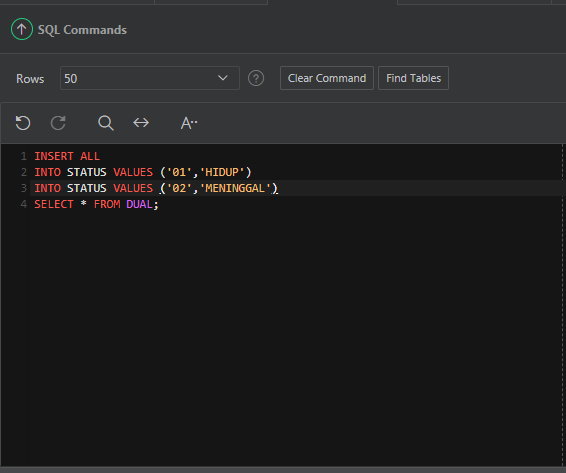
\includegraphics[width=13cm,height=7cm]{figures/F1.PNG}
\caption{Insert Into tabel STATUS}
\label{penanda}
\end{figure}
\item Selanjutnya kita melakukan Insert pada tabel SENSUS JLH PENDUDUK.
\begin{figure}[!htbp]
\centering
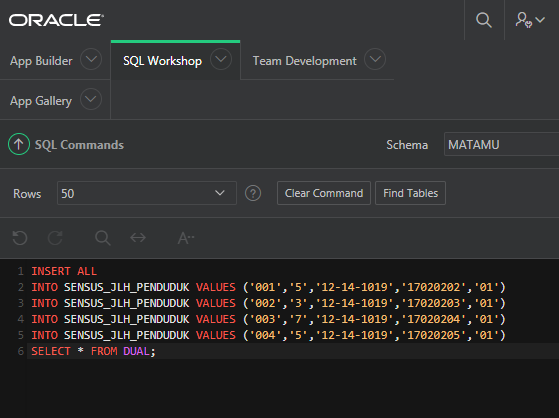
\includegraphics[width=13cm,height=8cm]{figures/G1.PNG}
\caption{Insert Into tabel SENSUS}
\label{penanda}
\end{figure}
\section{Pembuatan \textit{Trigger} dan\textit{View}}
\par Pengertian Trigger merupakan sekumpulan perintah atau sintaks yang akan secara otomatis dijalankan jika terjadi operasi tertentu dalam tabel atau view. Trigger digunakan untuk memanggil satu atau beberapa perintah SQL secara otomatis sebelum atau sesudah terjadi proses INSERT, UPDATE atau DELETE dari suatu tabel.
\par View adalah tabel virtual yang berisi data yang ditentukan berdasarkan query yang dibuat. Seperti tabel biasa, sebuah view terdiri dari kolom dan baris data. Namun view tidak menyimpan data dalam database karena view dibuat dari tabel-tabel yang telah ada dalam database. Sehingga data yang dimiliki oleh view adalah data-data yang mereferensi ke tabel lain sesuai dengan query dan akan berubah secara dinamis sesuai dengan isi data yang dijadikan reference-nya.
\item nah disini, kita membuat trigger pada Tabel STATUS JLH PENDUDUK contoh seperti dibawah ini.
\begin{figure}[!htbp]
\centering
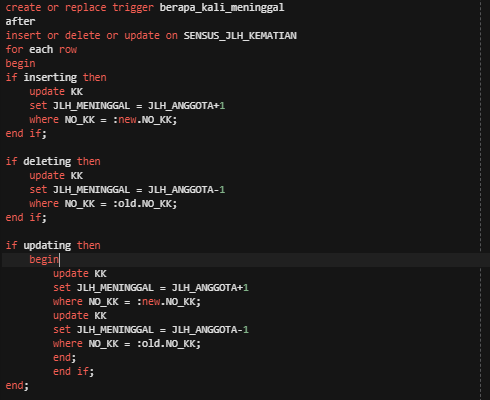
\includegraphics[width=13cm,height=11cm]{figures/H.PNG}
\caption{Trigger}
\label{penanda}
\end{figure}
\item Selanjutnya kita membuat View untuk menampilkan Pembaharuan pada Aplikasi nanti.
\begin{figure}[!htbp]
\centering
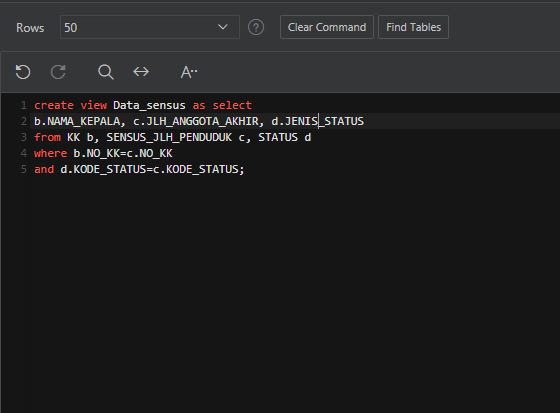
\includegraphics[width=13cm,height=7cm]{figures/H1.PNG}
\caption{View}
\label{penanda}
\end{figure}
\item Jika sudah, Kita Lakukan Percobaan Sesuai Keinginan Kita apakah Delete, Insert ataupun Update.
\item Setelah Itu Selesai Untuk Membuat Data Basenya.
\section{Membuat Aplikasi Sensus}
\par
\item Klik \textit{App Builder}
\begin{figure}[!htbp]
\centering
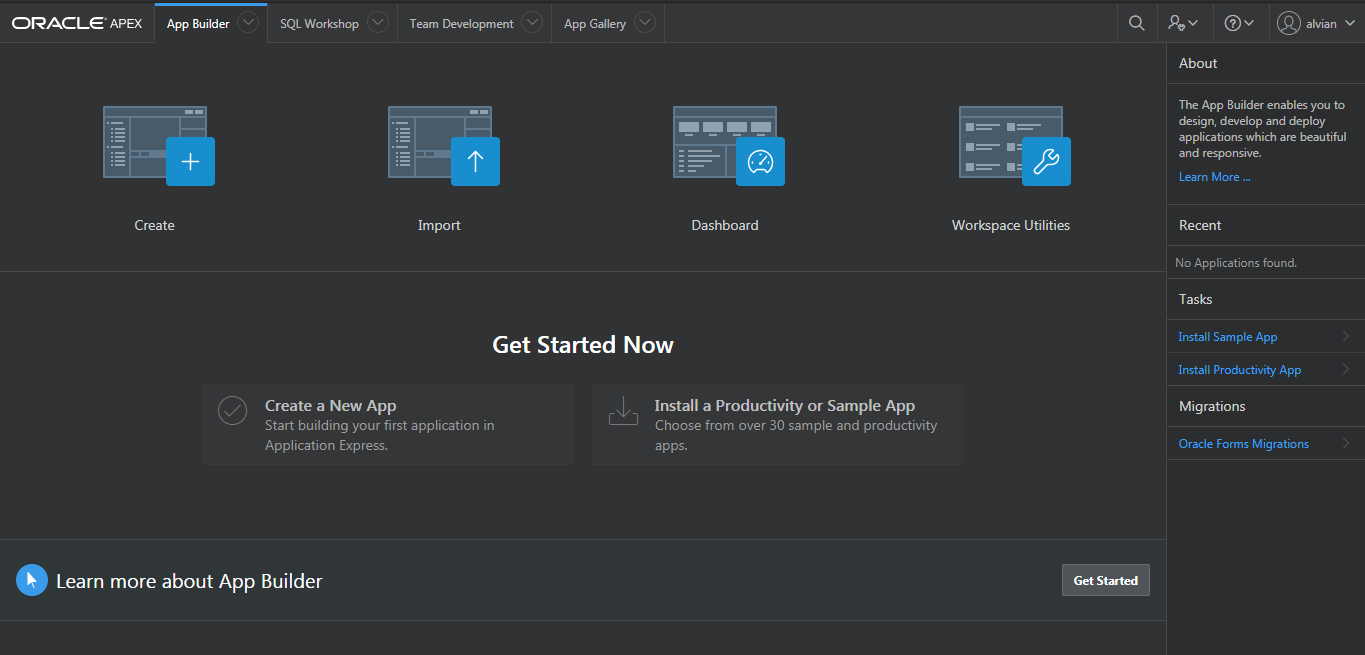
\includegraphics[width=13cm,height=7cm]{figures/app.PNG}
\caption{Klik App Builder}
\label{penanda}
\end{figure}
\item Lalu, Pilih \textit{CREATE}akan ditampilkan seperti gambar dibawah ini.
\begin{figure}[!htbp]
\centering
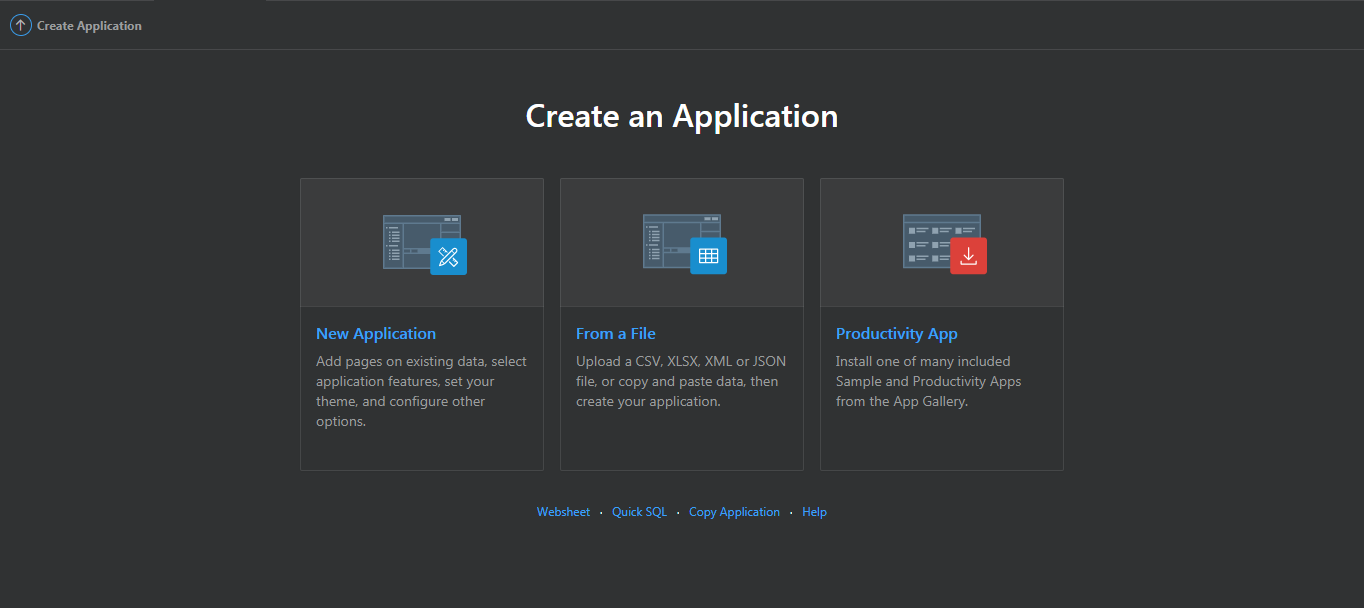
\includegraphics[width=13cm,height=8cm]{figures/H2.PNG}
\caption{Pilih Create}
\label{penanda}
\end{figure}
\item Kemudian, Klik \textit{New Application} 
\begin{figure}[!htbp]
\centering
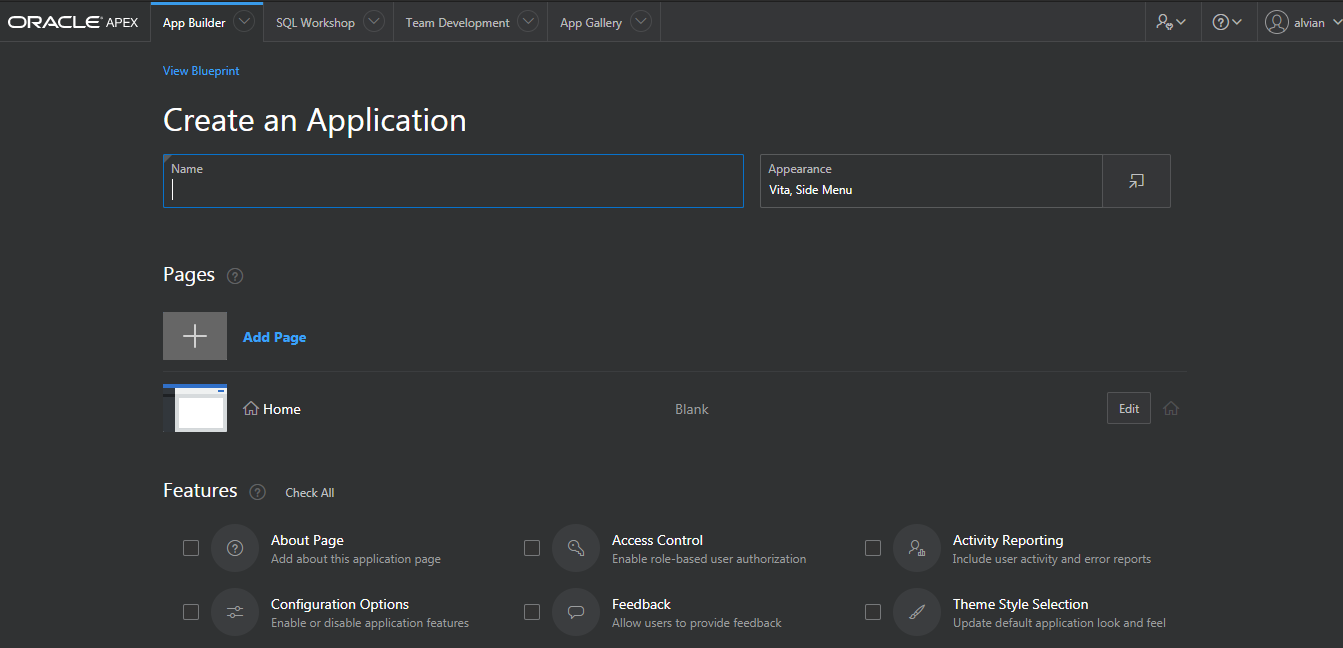
\includegraphics[width=13cm,height=8cm]{figures/H3.PNG}
\caption{New Application}
\label{penanda}
\end{figure}
\item Masukkan Nama Aplikasinya, disini saya membuat \textbf{aplikasi sensus Penduduk}.
\item Kemudian, pilih Page apa yang anda gunakan pada aplikasi, disini saya menggunakan \textit{Interactive Report}
\begin{figure}[!htbp]
\centering
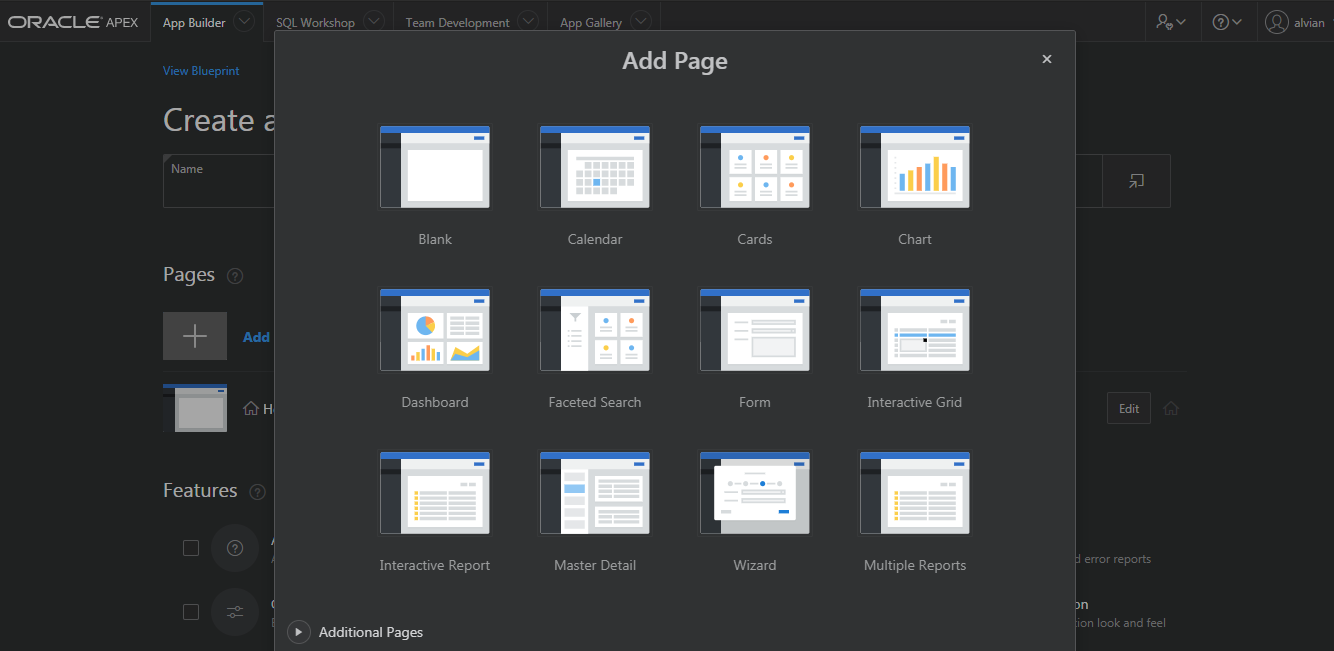
\includegraphics[width=13cm,height=8cm]{figures/H4.PNG}
\caption{Add Page}
\label{penanda}
\end{figure}
\item  Setelah itu, isi nama page dan masukkan tabel database yang kita buat tadi, disini saya memasukkan Nama page yaitu Kartu Keluarga dengan tabel KK.
\begin{figure}[!htbp]
\centering
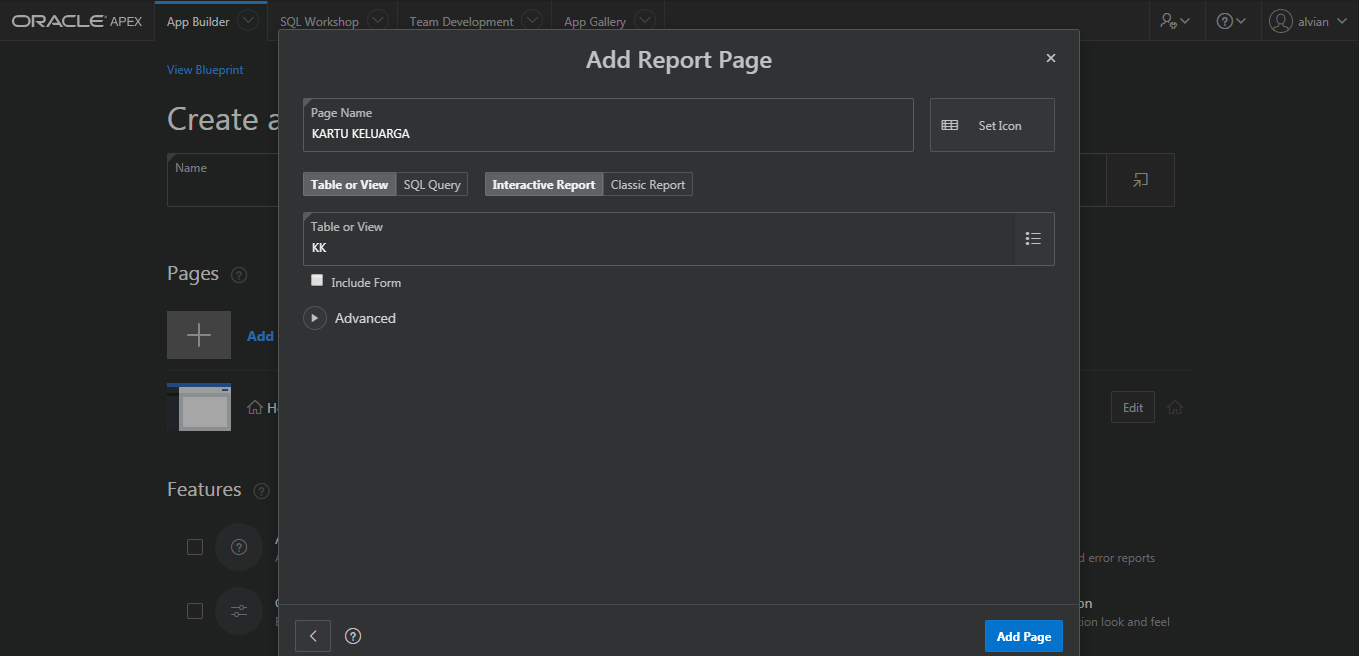
\includegraphics[width=13cm,height=8cm]{figures/H5.PNG}
\caption{Nama page dan Tabel}
\label{penanda}
\end{figure}
\item Lakukan hal yang sama diatas dari langkah NO 21-22 pada Tabel STATUS dan SENSUS JLH PENDUDUK.
\item Kemudian Kemudian akan seperti gambar dibawah ini.
\begin{figure}[!htbp]
\centering
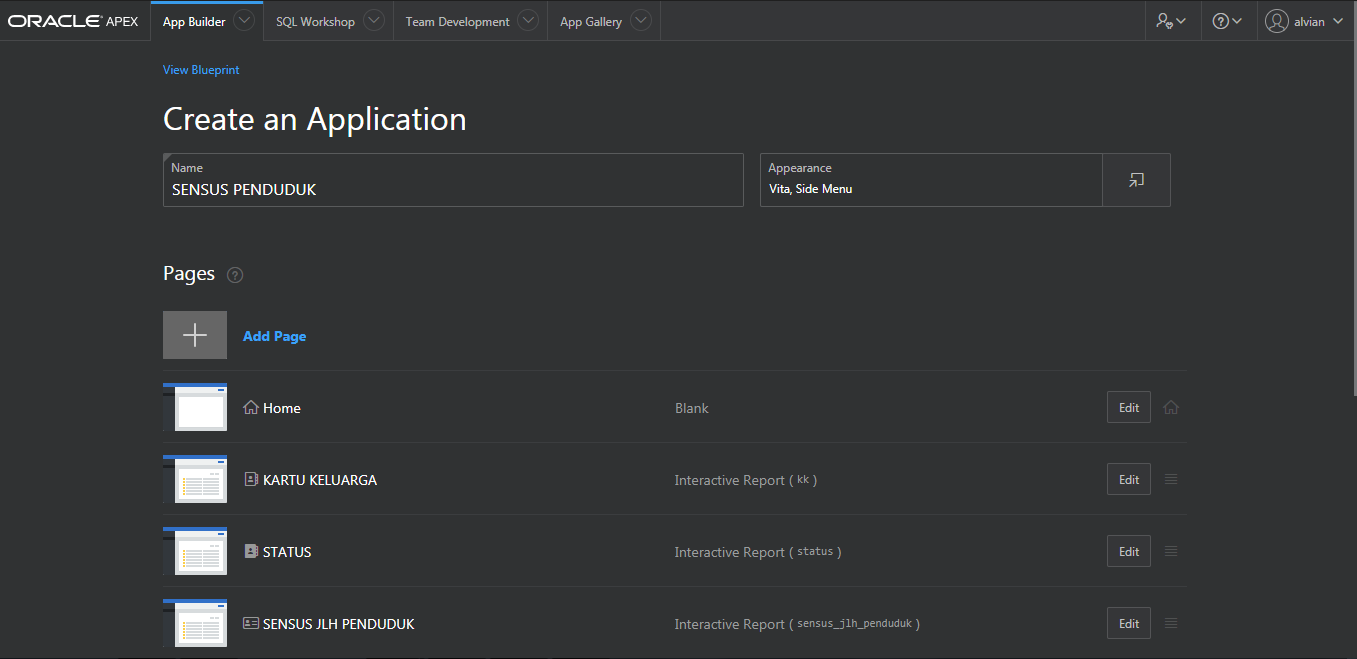
\includegraphics[width=13cm,height=7cm]{figures/H6.PNG}
\caption{Tampilan Akhir}
\label{penanda}
\end{figure}
\item  Scroll kebawah lalu klik create application.
\item Maka Aplikasi telah dibuat.
\begin{figure}[!htbp]
\centering
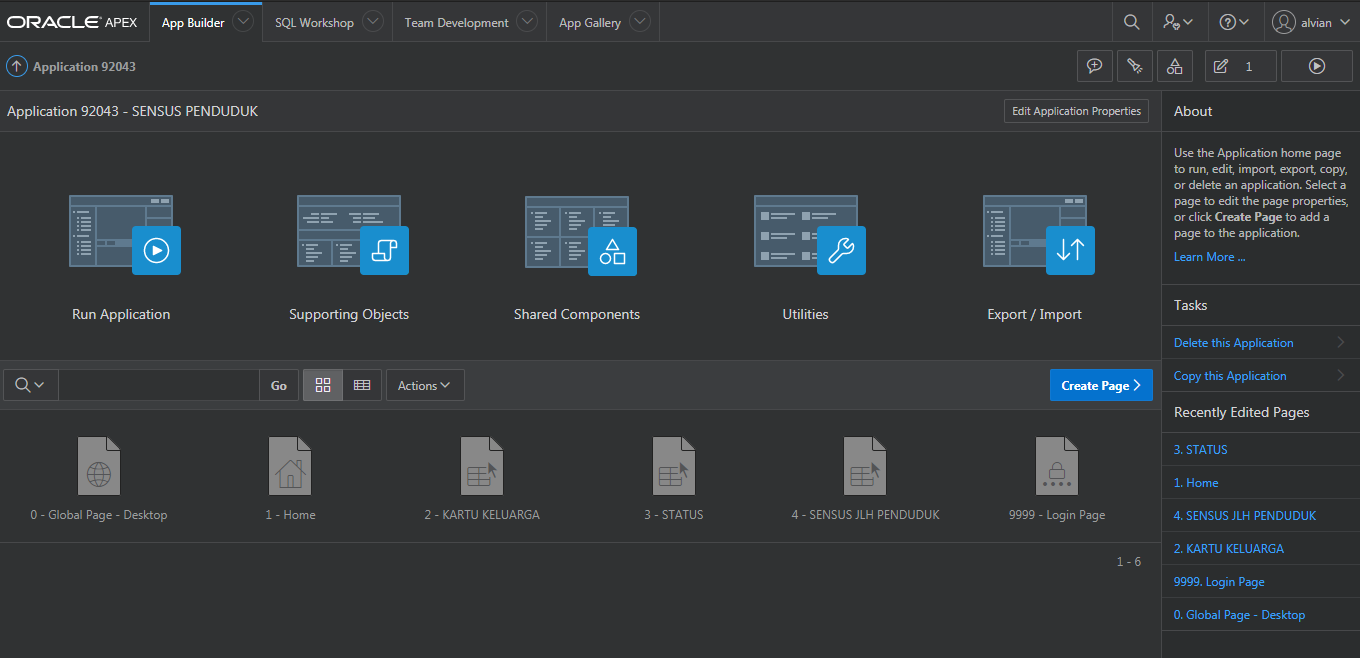
\includegraphics[width=13cm,height=8cm]{figures/H7.PNG}
\caption{Aplikasi telah dibuat}
\label{penanda}
\end{figure}
\item Pilih Run application.
\begin{figure}[!htbp]
\centering
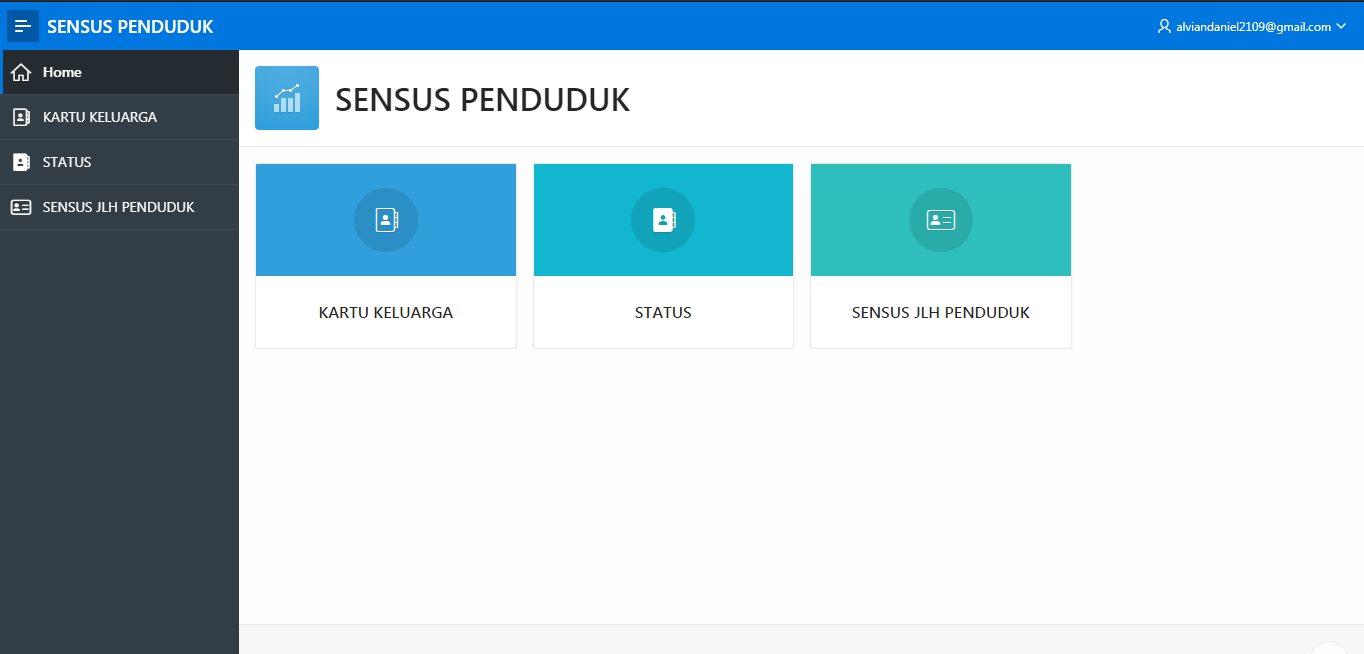
\includegraphics[width=13cm,height=8cm]{figures/H8.PNG}
\caption{Run application Sensus Penduduk}
\label{penanda}
\end{figure}
\end{enumerate}

